\documentclass{article}
\usepackage[utf8]{inputenc}
\usepackage[english]{babel}
\usepackage{biblatex}
\usepackage{amsmath}
\usepackage{amssymb}
\usepackage{caption}
\usepackage{subcaption}
\usepackage{graphicx}
\usepackage{csquotes}
\usepackage{booktabs}
\usepackage{lipsum}
\usepackage{setspace}
\usepackage[letterpaper,top=2cm,bottom=2cm,left=3cm,right=3cm,marginparwidth=1.75cm]{geometry}

% Font
\usepackage{charter}

% Hyperlink config
\usepackage{hyperref}
\hypersetup{
    colorlinks=true,
    linkcolor=blue,
    filecolor=magenta,      
    urlcolor=cyan,
    pdftitle={Overleaf Example},
    pdfpagemode=FullScreen,
}

% Code snippets
% \usepackage{minted}
\usepackage{minted}
\usepackage{xcolor}
\usepackage{caption}

\definecolor{codebg}{rgb}{0.95,0.95,0.95}
\definecolor{codeframe}{rgb}{0.75,0.75,0.75}

% Title and footnote
\usepackage{titling}
\newcommand{\subtitle}[1]{%
  \posttitle{%
    \par\end{center}
    \begin{center}\large#1\end{center}
    \vskip0.5em}%
}
\usepackage{hyperref}
\newcommand{\footremember}[2]{%
   \footnote{#2}
    \newcounter{#1}
    \setcounter{#1}{\value{footnote}}%
}

\renewcommand{\baselinestretch}{1.15}
\addbibresource{ref.bib}

\setlength{\parindent}{0em}
\setlength{\parskip}{0.5em}

\title{CS 5785 Homework 2}
\subtitle{Cornell Tech, Fall 2023}

\author{
    Tian Jin\thanks{\href{mailto:tj299@cornell.edu}{tj299@cornell.edu}. Tian mainly contributes to the Written Exercises.}
\and{
    Yufan Zhang\thanks{\href{mailto:yz2894@cornell.edu}{yz2894@cornell.edu}. Yufan mainly contributes to the Programming Exercises.}
}}

\date{September 2023}


% ======================
\begin{document}

\maketitle

\section{Binary Classification on Text Data}
\subsection{Basic Statistics of the Data}
In this \href{https://www.kaggle.com/competitions/nlp-getting-started/overview}{Kaggle competition}, we are given a dataset of 7613 tweets as training data and 3263 tweets as test data, each labeled as either a disaster or not. The goal is to build a binary classification model to predict whether a tweet is about a disaster or not. There are approximately 42.97\% (3271) of the tweets labeled as disaster and 57.03\% (4342) of the tweets labeled as not disaster in the training data. The test data is unlabeled and the prediction results will be evaluated by the accuracy of the prediction. Listing~\ref{code:basic} shows the code to get the basic statistics of the dataset.

\begin{listing}[H]
\caption{Code to get the basic statistics of the dataset}
\label{code:basic}
\begin{minted}[bgcolor=codebg, frame=lines, framesep=2mm, linenos]{python}
# Load the training and test data
def load_data_from_csv(filename):
    return pd.read_csv(os.path.join(DATA_PATH, filename), index_col=0)

# Load the train and test data
df = load_data_from_csv("train.csv")
X_test = load_data_from_csv("test.csv")

# Amount of data
print("The number of data points:")
print(f"training data \t {len(df)} \t test data \t {len(X_test)}\n")

# Percentage of classes
print("Percentage of training tweets are of real disasters:")
print(f"{round(df['target'].value_counts()[1]/len(df)*100, 2)}%")
print("Percentage of training tweets are not of real disasters:")
print(f"{round(df['target'].value_counts()[0]/len(df)*100, 2)}%")
\end{minted}
\end{listing}

\subsection{Splitting the Training Data}

We split the training data into training and development sets with a ratio of 0.7:0.3. The training set is used to train the model and the development set is used to evaluate the model. The code to split the training data is shown in Listing~\ref{code:split}.

\begin{listing}[H]
\caption{Code to split the training data}
\label{code:split}
\begin{minted}[bgcolor=codebg, frame=lines, framesep=2mm, linenos]{python}
# Split the training data w/o sklearn
def train_test_split(X, y, test_size=0.2, random_state=42):
    np.random.seed(random_state)
    shuffled_indices = np.random.permutation(len(X))
    test_set_size = int(len(X) * test_size)
    test_indices = shuffled_indices[:test_set_size]
    train_indices = shuffled_indices[test_set_size:]
    return (
        X.iloc[train_indices],
        X.iloc[test_indices],
        y.iloc[train_indices],
        y.iloc[test_indices],
    )
    
X = drop_features(df, ["target"])
y = keep_features(df, ["target"])

X_train, X_dev, y_train, y_dev = train_test_split(X, y, test_size=.3)

print(f"X_train: {X_train.shape} \t y_train: {y_train.shape}")
print(f"X_dev: {X_dev.shape} \t y_dev: {y_dev.shape}")

# X_train: (5330, 1) 	 y_train: (5330, 1)
# X_dev: (2283, 1) 	     y_dev: (2283, 1)
\end{minted}
\end{listing}

\subsection{Data Preprocessing}

\subsubsection{Handle hashtags}

In the first stage of the data preprocessing phase, special attention was given to the handling of hashtags. Hashtags often encapsulate key information but are written concatenated, such as “\#WorldNews". Since the objective is to extract meaningful features from the text using Bag-of-Words (BoW) and N-Gram models, it is essential to break down these hashtags into their constituent words. For example, the hashtag “\#WorldNews" would be split into “World" and “News". This allows the feature extraction methods to recognize and give appropriate weight to each individual term. Concurrently, the hashtag symbol “\#" is removed to ensure that the split words are treated the same way as other words in the tweet. Listing~\ref{code:hashtag} shows the code to handle hashtags.

\begin{listing}[H]
\caption{Code to handle hashtags}
\label{code:hashtag}
\begin{minted}[bgcolor=codebg, frame=lines, framesep=2mm, linenos]{python}
# Handle hashtags
def handle_hashtags(df):
    def split_hashtag_into_words(text):
        # Helper function to split words in hashtag
        return " ".join(re.findall(r"[A-Z]?[a-z]+|[A-Z]+(?=[A-Z]|$)", text))
        
    df["text"] = df["text"].apply(
        lambda x: re.sub(
            r"#(\S+)", lambda y: split_hashtag_into_words(y.group(1)), x
        )
    )
    return df
\end{minted}
\end{listing}


\subsubsection{Lowercase all text}

The next step in our data preprocessing pipeline is to convert all the text within the tweet data to lowercase. This is done to ensure uniformity and to eliminate any case-based discrepancies that could affect the feature extraction and the subsequent machine learning model. For example, the words “Science," “SCIENCE," and “science" may appear differently to a computer algorithm, but they all signify the same concept. This simple yet impactful modification aids in creating a more robust feature set for the machine learning algorithms to leverage. Listing~\ref{code:lowercase} shows the code to lowercase all text.

\begin{listing}[H]
\caption{Code to lowercase all text}
\label{code:lowercase}
\begin{minted}[bgcolor=codebg, frame=lines, framesep=2mm, linenos]{python}
# Lowercase all text
def convert_to_lowercase(df):
    df["text"] = df["text"].str.lower()
    return df
\end{minted}
\end{listing}


\subsubsection{Strip URLs and Mentions}

The next step is the removal of URLs and mentions from the tweet text data. URLs often do not contribute meaningful information for text classification in the context of our project, and they may introduce noise that hampers the effectiveness of the machine learning models. Similarly, mentions—indicated by the “@" symbol followed by a username—are usually specific to individual users and do not add generalizable value to the classification task. Therefore, both URLs and mentions are extracted and removed from the tweets during this preprocessing phase. By eliminating these elements, we aim to simplify the text data and focus on the words and phrases that are most relevant for accurate classification. This step enhances the clarity of the dataset, making it easier for the Bag-of-Words and N-Gram models to identify meaningful features. Listing~\ref{code:url} shows the code to strip URLs and mentions.

\begin{listing}[H]
\caption{Code to strip URLs and mentions}
\label{code:url}
\begin{minted}[bgcolor=codebg, frame=lines, framesep=2mm, linenos]{python}
# Strip @ and urls.
def strip_mentions_and_urls(df):
    def helper(text):
        # Remove @mentions
        text = re.sub(r"@\w+", "", text)
        # Remove URLs
        text = re.sub(r"http\S+", "", text)
        return text

    df["text"] = df["text"].apply(helper)
    return df
\end{minted}
\end{listing}


\subsubsection{Lemmatization}

The subsequent step involves the lemmatization of words using the \href{https://www.nltk.org/}{Natural Language Toolkit (nltk)}. Lemmatization is the process of converting words into their base or root form, which aids in reducing the dimensionality of the feature space. For example, the words ‘running', ‘runs' and ‘ran' would all be simplified to their lemma, ‘run'. This is particularly important for our project, as we aim to perform text classification using BoW and N-Gram models. Listing~\ref{code:lemmatization} shows the code to lemmatize words.

\begin{listing}[H]
\caption{Code to lemmatize words}
\label{code:lemmatization}
\begin{minted}[bgcolor=codebg, frame=lines, framesep=2mm, linenos]{python}
# Lemmatize all the words
def lemmatize_words(df):
    lemmatizer = WordNetLemmatizer()
    df["text"] = df["text"].apply(
        lambda x: " ".join(
            [lemmatizer.lemmatize(word) for word in word_tokenize(x)]
        )
    )
    return df
\end{minted}
\end{listing}


\subsubsection{Remove punctuation}

The next step is the removal of punctuation marks from the tweet text. Punctuation often adds structural complexity but usually does not contribute to the semantic meaning when text data is analyzed using Bag-of-Words and N-Gram models. By stripping the text of the punctuation marks, we create a cleaner, more uniform dataset that is easier to work with. Listing~\ref{code:punctuation} shows the code to remove punctuation.

\begin{listing}[H]
\caption{Code to remove punctuation}
\label{code:punctuation}
\begin{minted}[bgcolor=codebg, frame=lines, framesep=2mm, linenos]{python}
# Strip punctuation
def strip_punctuation(df):
    df["text"] = df["text"].str.replace(r'[^\w\s]', "", regex=True)
    return df
\end{minted}
\end{listing}


\subsubsection{Remove non-alphabetic characters}

The next preprocessing step entails the removal of all non-alphabetic characters from the tweet text. This includes numerical digits and any special characters that have not already been eliminated in earlier steps. The rationale behind this action is to focus solely on the words for our text classification task, as we are utilizing Bag-of-Words and N-Gram models for feature extraction. Non-alphabetic characters can introduce noise and complexity into the dataset without contributing meaningful information for classification. Listing~\ref{code:non-alphabetic} shows the code to remove non-alphabetic characters.

\begin{listing}[H]
\caption{Code to remove non-alphabetic characters}
\label{code:non-alphabetic}
\begin{minted}[bgcolor=codebg, frame=lines, framesep=2mm, linenos]{python}
# Remove latin characters and digits
def remove_latin_and_digits(df):
    df["text"] = df["text"].str.replace(r"[^a-zA-Z\s]", "", regex=True)
    return df
\end{minted}
\end{listing}


\subsubsection{Remove stopwords}

The subsequent stage involves the removal of stopwords using the mltk. Stopwords are commonly occurring words such as ‘and,' ‘the,' and ‘is', which, although essential for human communication, usually do not provide significant information for text classification tasks. Given our aim to use Bag-of-Words and N-Gram models for feature extraction, eliminating these high-frequency but low-impact words is beneficial. Listing~\ref{code:stopwords} shows the code to remove stopwords.

\begin{listing}[H]
\caption{Code to remove stopwords}
\label{code:stopwords}
\begin{minted}[bgcolor=codebg, frame=lines, framesep=2mm, linenos]{python}
# Strip the stop words, e.g., "the”, "and”, "or”
def strip_stopwords(df):
    stop = stopwords.words("english")
    df["text"] = df["text"].apply(
        lambda x: " ".join(x for x in x.split() if x not in stop)
    )
    return df
\end{minted}
\end{listing}

\subsubsection{Streamline data preprocessing pipeline}

To streamline the data preprocessing workflow and ensure consistent treatment of all tweet texts, we have encapsulated all the individual preprocessing steps into a single function named `data\_preprocess`. This function takes a DataFrame as input and sequentially applies each preprocessing operation, from handling hashtags and converting text to lowercase, to removing mentions, URLs, and stopwords. Other operations such as lemmatization, punctuation removal, and the elimination of non-alphabetic characters are also conducted in this unified function. The processed DataFrame is then returned, ready for feature extraction and subsequent analysis. By consolidating all preprocessing steps into a single function, we achieve greater efficiency and maintainability to iterate on our machine learning models. Listing~\ref{code:preprocess} shows the code to streamline the data preprocessing pipeline.

\begin{listing}[H]
\caption{Code for streamlined data preprocess}
\label{code:preprocess}
\begin{minted}[bgcolor=codebg, frame=lines, framesep=2mm, linenos]{python}
# Combine all the preprocessing steps into a single function
def data_preprocess(df):
    df = handle_hashtags(df)
    df = convert_to_lowercase(df)
    df = strip_mentions_and_urls(df)
    df = lemmatize_words(df)
    df = strip_punctuation(df)
    df = remove_latin_and_digits(df)
    df = strip_stopwords(df)
    return df
\end{minted}
\end{listing}


\subsection{Bag of Words Model}

In the Bag-of-Words (BoW) model, each tweet is represented by a feature vector \( \textbf{x} \) of length equal to the size of the vocabulary created from the dataset. The entry at the \( i^{th} \) position of the feature vector is set to 1 if the corresponding \( i^{th} \) vocabulary word appears in the tweet; otherwise, it remains 0. To manage computational and memory efficiency, as well as to eliminate noisy or unreliable features, we implemented a minimum document frequency threshold, termed \texttt{min\_df}.

To determine the appropriate value for \texttt{min\_df}, we followed these steps:

\begin{itemize}
    \item \textbf{Start with a Small Value:} Initially set \texttt{min\_df} to a 1 to include all terms in the vocabulary.
    
    \item \textbf{Build and Evaluate the Model:} With this initial \texttt{min\_df} value, train a logistic regression model with L2 regularization. Evaluate the model's performance (i.e., F1-score) on a validation set.
    
    \item \textbf{Iterate and Increase \texttt{min\_df}:} Gradually increase the value of \texttt{min\_df} and retrain and re-evaluate the model. Keep track of how the model's performance changes.
    
    \item \textbf{Final Value:} The optimal \texttt{min\_df} value would be the one resulting in the highest F1-score.
\end{itemize}

\begin{figure}[!htbp]
    \centering
    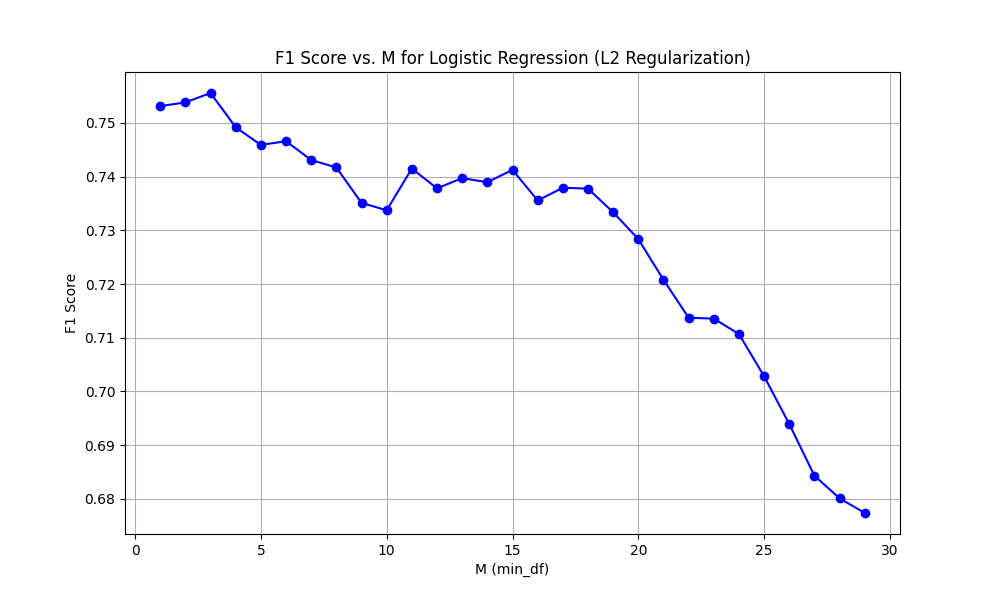
\includegraphics[width=\textwidth]{img/f1_score_vs_m_bow.png}
    \caption{F1-score vs. \texttt{min\_df} in BoW model}
    \label{fig:bow-min_df}
\end{figure}

Throughout this iterative process, we noted the effect of increasing \texttt{min\_df} on the model's performance. As \texttt{min\_df} increased, the vocabulary size reduced, effectively filtering out terms that appeared in fewer tweets. By closely monitoring the F1-score, we found that the optimal \texttt{min\_df} value was \textbf{3}, at which the model yielded the highest F1-score. As Figure~\ref{fig:bow-min_df} shows, the F1-score increased as \texttt{min\_df} increased from 1 to 3, but it decreased as \texttt{min\_df} increased after 3. This indicates that terms appearing in fewer than three tweets may have been adding noise rather than useful information. Therefore, setting \texttt{min\_df} to 3 provided us with a reliable, efficient feature set for subsequent modeling and analysis. Listing~\ref{code:bow-min_df} shows the code to implement such an iterative process to find the optimal \texttt{min\_df} value.

Before going further and implementing the classification models, we first constructed a function named \texttt{infer\_and\_save\_result} to streamline the evaluation of various models. This function takes several parameters, including the model name, vectorizer, training and development datasets, and performs several tasks. Initially, it transforms the text data into feature vectors using the supplied vectorizer. Subsequently, it infers the labels for both the training and development sets and calculates their respective macro-averaged F1 scores. Finally, the function saves essential components such as the vectorizer, the trained model, and the F1 scores for both datasets in a dictionary for easy comparison later. Listing~\ref{code:infer-save} shows the code to implement \texttt{infer\_and\_save\_result}.

\begin{listing}[H]
\caption{Code for iterative process to find the optimal \texttt{min\_df} value}
\label{code:bow-min_df}
\begin{minted}[bgcolor=codebg, frame=lines, framesep=2mm, linenos]{python}
# Find the M with the highest F1 score
# Initialize empty lists to store values
M_values = []
F1_scores = []

# Find the M with the highest F1 score
for M in range(1, 30, 1):
    # Initialize the CountVectorizer with binary=True and min_df=M
    vectorizer = CountVectorizer(binary=True, min_df=M)

    # Vectorize the X_train
    X_train_bow_matrix = vectorizer.fit_transform(X_train['text'])
    X_train_bow = pd.DataFrame(
        X_train_bow_matrix.toarray(), columns=vectorizer.get_feature_names_out()
    )
    
    # Initialize and train the model
    model = LogisticRegression(penalty="l2", max_iter=1000)
    model.fit(X_train_bow, y_train)

    # Predict the labels of the validation set
    y_pred = model.predict(vectorizer.transform(X_dev['text']))
    score = f1_score(y_dev, y_pred)

    # Append M and its corresponding F1 score to the lists
    M_values.append(M)
    F1_scores.append(score)
    
    
# Create a plot
plt.figure(figsize=(10, 6))
plt.plot(M_values, F1_scores, marker='o', linestyle='-', color='b')
plt.title("F1 Score vs. M for Logistic Regression (L2 Regularization)")
plt.xlabel("M (min_df)")
plt.ylabel("F1 Score")
plt.grid(True)
plt.savefig(os.path.join(IMG_PATH, "f1_score_vs_m_bow.png"))
plt.show()

# Get the index of the M with the highest F1 score
best_M = np.argmax(F1_scores)
print(f"Best value for M: {M_values[best_M]}")

# Best value for M: 3
\end{minted}
\end{listing}

\begin{listing}[H]
\caption{Code for \texttt{infer\_and\_save\_result}}
\label{code:infer-save}
\begin{minted}[bgcolor=codebg, frame=lines, framesep=2mm, linenos]{python}
# Record trained models and their results
models = dict()

def infer_and_save_result(
    model_name, vectorizer, model, X_train, y_train, X_dev, y_dev
):
    print(model_name)
    X_train_vec = vectorizer.transform(X_train['text'])
    X_train_vec = pd.DataFrame(
        X_train_vec.toarray(), columns=vectorizer.get_feature_names_out()
    )
    X_dev_vec = vectorizer.transform(X_dev['text'])
    X_dev_vec = pd.DataFrame(
        X_dev_vec.toarray(), columns=vectorizer.get_feature_names_out()
    )

    # Infer the training set
    y_pred_train = model.predict(X_train_vec)
    # Calculate the F1 score
    f1_train = f1_score(y_train, y_pred_train, average="macro")
    print("F1 score on training set: {:.4f}".format(f1_train))

    # Infer the dev set
    y_pred_dev = model.predict(X_dev_vec)
    # Calculate the F1 score
    f1_dev = f1_score(y_dev, y_pred_dev, average="macro")
    print("F1 score on dev set: {:.4f}".format(f1_dev))

    # Save the result
    models[model_name] = {
        "vectorizer": vectorizer,
        "model": model,
        "f1_train": f1_train,
        "f1_dev": f1_dev,
    }
\end{minted}
\end{listing}


\subsection{Logistic Regression}

We employ the results of BoW models to evaluate three logistic regression models: one without regularization, one with L1 regularization, and one with L2 regularization. The resulting performance on training and development sets are shown in Table~\ref{tab:results-lr-bow}. We can see that the model with L2 regularization performs the best on the development set, with an F1-score of 0.7955. Listing~\ref{code:lr-bow} shows the code to implement the logistic regression models.

\begin{table}[h]
    \centering
    \begin{tabular}{|c|c|c|}
        \hline
        \textbf{Model} & \textbf{F1 Score on Training Set} & \textbf{F1 Score on Dev Set} \\
        \hline
        Logistic Regression (Without Regularization) & 0.9813 & 0.7084 \\
        \hline
        Logistic Regression (L1 Regularization) & 0.8718 & 0.7878 \\
        \hline
        Logistic Regression (L2 Regularization) & 0.9066 & 0.7955 \\
        \hline
    \end{tabular}
    \caption{F1 Scores for Different Logistic Regression Models with BoW}
    \label{tab:results-lr-bow}
\end{table}

\begin{listing}[H]
\caption{Code for logistic regression models}
\label{code:lr-bow}
\begin{minted}[bgcolor=codebg, frame=lines, framesep=2mm, linenos]{python}
# Train a logistic regression without regularization
model = LogisticRegression(penalty="none", max_iter=1000)
model.fit(X_train_bow, y_train)

infer_and_save_result(
    "Logistic Regression (Without Regularization) with BoW",
    vectorizer, model,
    X_train, y_train, X_dev, y_dev,
)

# Train a logistic regression with L1 regularization
model = LogisticRegression(penalty="l1", max_iter=1000)
model.fit(X_train_bow, y_train)

infer_and_save_result(
    "Logistic Regression (L1 Regularization) with BoW",
    vectorizer, model,
    X_train, y_train, X_dev, y_dev,
)

# Train a logistic regression with L2 regularization
model = LogisticRegression(penalty="l2", max_iter=1000)
model.fit(X_train_bow, y_train)

infer_and_save_result(
    "Logistic Regression (L2 Regularization) with BoW",
    vectorizer, model,
    X_train, y_train, X_dev, y_dev,
)
\end{minted}
\end{listing}

After fitting the logistic regression models, we took a closer look at the model utilizing L1 regularization to inspect its weight vector, commonly denoted as \(\theta\). L1 regularization effectively zeroes out irrelevant features, making it ideal for feature selection. To examine the importance of each feature, we accessed the \texttt{coef\_} attribute of the trained \texttt{LogisticRegression} instance to retrieve the weight vector. We then paired these coefficients with their corresponding feature names and sorted them by their absolute values in descending order.

\begin{table}[h]
\centering
\begin{tabular}{|c|c|}
\hline
\textbf{Feature} & \textbf{Coefficient} \\
\hline
hiroshima & 3.4721 \\
spill & 3.3908 \\
typhoon & 3.2693 \\
airport & 3.2259 \\
migrant & 3.1984 \\
derailment & 3.1836 \\
wildfire & 3.1072 \\
earthquake & 2.9806 \\
debris & 2.9161 \\
outbreak & 2.8898 \\
\hline
\end{tabular}
\caption{Top 10 words for predicting a real disaster}
\label{table:top-10-words}
\end{table}

The table \ref{table:top-10-words} shows the top 10 words that have the highest absolute coefficients, suggesting that these words are strong indicators for predicting real disasters in tweets. Words like “hiroshima", “spill," and “typhoon" are naturally associated with events of serious consequence, which validates the model's focus on these terms. The presence of such strong, unambiguous indicators in the weight vector underscores the model's capability to pick out the most significant words for the classification task. This inspection thus provides not just a sanity check for our model but also potentially valuable insights into the characteristics of tweets that are most indicative of real disasters. Listing~\ref{code:top-10-words} shows the code to get the top 10 words for predicting a real disaster.

\begin{listing}[H]
\caption{Code for getting the top 10 words for predicting a real disaster}
\label{code:top-10-words}
\begin{minted}[bgcolor=codebg, frame=lines, framesep=2mm, linenos]{python}
# Get the L1 regularization logistic regression model
model_dict = models["Logistic Regression (L1 Regularization) with BoW"]
model = model_dict["model"]
fea_names = model_dict["vectorizer"].get_feature_names_out()

# Get the weight vector of the classifier
coefficients = model.coef_[0]

# Pair feature names with their coefficients
fea_coef = zip(fea_names, coefficients)

# Sort the features by their absolute coefficients in descending order
sorted_features = sorted(fea_coef, key=lambda x: abs(x[1]), reverse=True)

# Print the most important words/features
num_top_words = 10  # You can adjust this to show more or fewer top words
print(f"Top {num_top_words} words for predicting a real disaster:")
for feature, coef in sorted_features[:num_top_words]:
    print(f"{feature}: {coef}")
\end{minted}
\end{listing}

In addition to the logistic regression models, we also implemented a Bernoulli Naive Bayes classifier with Laplace smoothing. The classifier was built from scratch and applied to the feature vectors generated by our optimized Bag-of-Words (BoW) model. Laplace smoothing was employed to account for possible zero probabilities when estimating the conditional probabilities for each class label. This approach makes the Naive Bayes model more robust, particularly when dealing with features that may not appear in the training set but are present in the development set. Listing~\ref{code:naive-bayes} shows the code to implement the Bernoulli Naive Bayes classifier.

\begin{listing}[H]
\caption{Code for Bernoulli Naive Bayes classifier}
\label{code:naive-bayes}
\begin{minted}[bgcolor=codebg, frame=lines, framesep=2mm, linenos]{python}
class BernoulliNaiveBayes:
    def __init__(self, alpha=1.0):
        self.alpha = alpha  # Laplace smoothing parameter
        self.d = None       # Number of features
        self.K = None       # Unique class labels
        self.psis = None    # Parameters of the Bernoulli distributions
        self.phis = None    # Class priors

    def fit(self, X, y):
        self.K = np.unique(y).shape[0]
        n = X.shape[0]  # Number of data points
        self.d = X.shape[1]
        self.psis = np.zeros([self.K, self.d])
        self.phis = np.zeros([self.K])

        for k in range(self.K):     # Update the parameters
            X_k = X[np.array(y_train == k)[:, 0]]
            self.psis[k] = (X_k.sum(axis=0) + self.alpha) / float(
                X_k.shape[0] + 2 * self.alpha
            )
            self.phis[k] = X_k.shape[0] / float(n)

    def predict(self, x):
        # adjust shapes
        n, d = x.shape
        x = np.reshape(x, (1, n, self.d))
        psis = np.reshape(self.psis, (self.K, 1, d))

        psis = psis.clip(1e-14, 1 - 1e-14)  # clip probabilities to avoid log(0)

        # compute log-probabilities
        logpy = np.log(self.phis).reshape([self.K, 1])
        logpxy = x * np.log(psis) + (1 - x) * np.log(1 - psis)
        logpyx = logpxy.sum(axis=2) + logpy

        return logpyx.argmax(axis=0).flatten()

# Make predictions on the dev set
bayes = BernoulliNaiveBayes()
bayes.fit(X_train_bow, y_train)
infer_and_save_result(
    "Bernoulli Naive Bayes with BoW",
    vectorizer, bayes, X_train, y_train, X_dev, y_dev,
)
\end{minted}
\end{listing}

The performance of the Bernoulli Naive Bayes model was evaluated using the F1 score, a balanced measure of precision and recall. On the training set, the model achieved an F1 score of 0.8481. When applied to the development set, the F1 score was 0.7963, which suggests that the model generalizes well to unseen data. These results validate the effectiveness of Bernoulli Naive Bayes when paired with an optimized BoW representation, making it a viable alternative to logistic regression for this classification task. Table~\ref{tab:results-nb-bow} shows the results of the Bernoulli Naive Bayes model.

\begin{table}[h]
    \centering
    \begin{tabular}{|c|c|c|}
        \hline
        \textbf{Model} & \textbf{F1 Score on Training Set} & \textbf{F1 Score on Dev Set} \\
        \hline
        Bernoulli Naive Bayes on BoW & 0.8481 & 0.7963 \\
        \hline
    \end{tabular}
    \caption{F1 Scores for Bernoulli Naive Bayes Model with BoW}
    \label{tab:results-nb-bow}
\end{table}


\subsection{Model Comparison}

Based on the F1 scores, the Bernoulli Naive Bayes model with an F1 score of 0.7963 on the development set performed comparably to the Logistic Regression model with L2 Regularization, which had an F1 score of 0.7955 on the development set. Both models performed well in predicting whether a tweet is related to a real disaster or not, but the \textbf{Naive Bayes model slightly outperformed the logistic models} on the development set, despite having a lower F1 score on the training set. This suggests that the \textbf{Naive Bayes model may generalize better to unseen data} in this specific task.

Regarding the pros and cons of generative versus discriminative models: generative models like Naive Bayes are often easier to train and require fewer data to make reasonable predictions. They model the underlying probability distribution of the data, which can be an advantage when you need to generate new samples. However, \textbf{they make strong assumptions about feature independence}. Discriminative models like Logistic Regression, on the other hand, focus on the boundary between classes and often achieve better performance when there is sufficient data. However, they may require more data to generalize well and are computationally more intensive to train.

Naive Bayes assumes that all features are conditionally independent given the class label. This is often \textbf{not the case in natural language processing tasks}, where word order and context can be important. Logistic regression does not make this independence assumption, instead, it models the probability that a given instance belongs to a particular category. Given these considerations, it appears valid and efficient to use a Bernoulli Naive Bayes classifier for natural language texts, especially when we have a smaller dataset, including this one. 
 

\subsection{N-gram Model}

After exploring feature extraction using the Bag-of-Words (BoW) model, we extended our investigation to incorporate N-Grams, specifically 2-Grams, into our feature vectors. Similar to the BoW model, we first determined the optimal value for \texttt{min\_df} for the 2-Gram \texttt{CountVectorizer}. This was achieved by running a logistic regression model on feature vectors generated with various \texttt{min\_df} values and monitoring the F1 score on the development set. Figure~\ref{fig:ngram-min_df} shows the F1 score for different \texttt{min\_df} values. After this empirical evaluation, the optimal \texttt{min\_df} was identified as 2. Listing~\ref{code:ngram-min_df} shows the code to find the optimal \texttt{min\_df} value for the 2-Gram \texttt{CountVectorizer}.


\begin{figure}[!htbp]
    \centering
    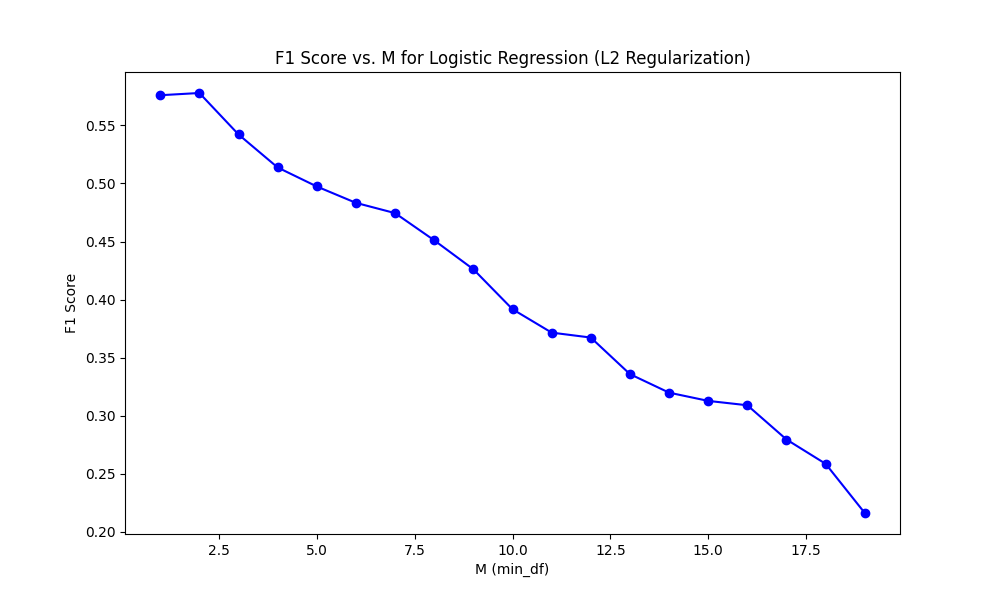
\includegraphics[width=0.9\textwidth]{img/f1_score_vs_m_ngram.png}
    \caption{F1-score vs. \texttt{min\_df} in 2-Gram model}
    \label{fig:ngram-min_df}
\end{figure}

\begin{listing}[H]
\caption{Code for finding the optimal \texttt{min\_df} value for the 2-Gram CountVectorizer}
\label{code:ngram-min_df}
\begin{minted}[bgcolor=codebg, frame=lines, framesep=2mm, linenos]{python}
M_values = []
F1_scores = []

# Find the M with the highest F1 score
for M in range(1, 20, 1):
    # CountVectorizer with min_df=M
    vectorizer = CountVectorizer(binary=True, min_df=M, ngram_range=(2, 2))
    X_train_bow_matrix = vectorizer.fit_transform(X_train['text']).toarray()
    
    # Initialize and train the model
    model = LogisticRegression(penalty="l2", max_iter=1000)
    model.fit(X_train_bow, y_train)

    # Predict the labels of the validation set
    y_pred = model.predict(vectorizer.transform(X_dev['text']))
    score = f1_score(y_dev, y_pred)

    M_values.append(M)
    F1_scores.append(score)
    
plt.figure(figsize=(10, 6))
plt.plot(M_values, F1_scores, marker='o', linestyle='-', color='b')
plt.title("F1 Score vs. M for Logistic Regression (L2 Regularization)")
plt.xlabel("M (min_df)")
plt.ylabel("F1 Score")
plt.savefig(os.path.join(IMG_PATH, "f1_score_vs_m_ngram.png"))
\end{minted}
\end{listing}


Utilizing this optimized \texttt{min\_df}, we employed scikit-learn's \texttt{CountVectorizer} to generate 2-Gram feature vectors. Subsequently, we assessed the performance of three logistic regression models—without regularization, with L1 regularization, and with L2 regularization—alongside a Bernoulli Naive Bayes model on these feature vectors. The code snippets similar to the ones shown in Listing~\ref{code:lr-bow}, although omitted here for brevity, encapsulate the core logic for this part of the experimentation. Upon evaluation, the performance metrics revealed a varied outcome. Table~\ref{tab:results-ngram} shows the results of the N-Gram models.

\begin{table}[h]
    \centering
    \begin{tabular}{|c|c|c|}
        \hline
        \textbf{Model} & \textbf{F1 Score on Training Set} & \textbf{F1 Score on Dev Set} \\
        \hline
        Logistic Regression (Without Regularization) & 0.8281 & 0.6950 \\
        \hline
        Logistic Regression (L1 Regularization) & 0.7395 & 0.6670 \\
        \hline
        Logistic Regression (L2 Regularization) & 0.7913 & 0.6910 \\
        \hline
        Bernoulli Naive Bayes & 0.7216 & 0.6430 \\
        \hline
    \end{tabular}
    \caption{F1 Scores for Different Models with 2-Gram}
    \label{tab:results-ngram}
\end{table}

This exercise highlights that while N-Gram features can capture more context than individual words alone, they did not necessarily improve classification performance in our case, particularly when compared to the BoW model. It suggests that, for this specific task, simpler BoW features may suffice.


\subsection{Performance on the Test Set}

Upon concluding the series of experiments on feature extraction methods and classifiers, we identified the Bernoulli Naive Bayes model with Bag-of-Words (BoW) features as the top-performing model. Accordingly, we re-trained this model using the entire training dataset and then tested its performance on the Kaggle test set. The result was an F1 score of 0.79895, which positioned us at rank 477 out of 987 on the Kaggle leaderboard. Figure~\ref{fig:kaggle-score} shows the Kaggle score.

\begin{figure}[!htbp]
    \centering
    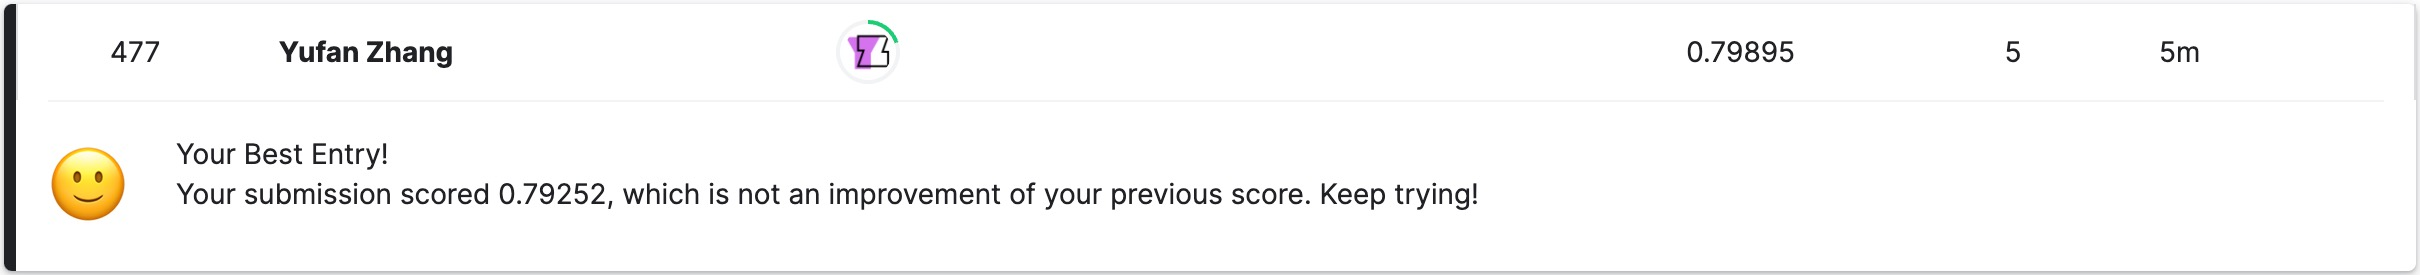
\includegraphics[width=\textwidth]{img/kaggle_result.jpg}
    \caption{Kaggle score}
    \label{fig:kaggle-score}
\end{figure}

Interestingly, the performance on the Kaggle test set slightly exceeded our expectations based on the development set results, where the F1 score was 0.7963. There are several factors that could account for this discrepancy. One possible explanation is that the Kaggle test set might contain examples that are more aligned with the feature representations learned by our model. Additionally, using the entire training set to re-train the model could have provided it with a more comprehensive understanding of the feature space, thus boosting its ability to generalize well to unseen data. This slight increase in performance on the Kaggle test set can be considered as a positive indicator of the model's reliability and generalization capability.


\section{Written Exercises}

\subsection{Naive Bayes with Binary Features}

\subsection{Categorical Naive Bayes}

\end{document}